In 1993 Smithey et. al. reported making an experimental determination of a single-mode of the vacuum state's electrical field \cite{Smithey}. In addition to making a bare measurement of the electrical field they, also, measured a squeezed state of the vacuum electrical field. Note that their approach was optical and that they used a slightly different form of the Wigner function than is proposed by Leonhardt (given earlier) : $W(x,p)=\frac{1}{\pi}\int\limits_{-\infty}^{\infty}\bra{x+x'}\rho\ket{x-x'}e^{-2ipx'}dx'$.

\begin{figure}%
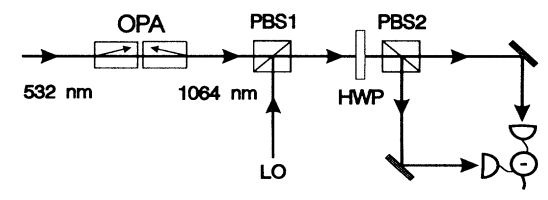
\includegraphics[width=274px,height=100px]{Figures/SmitheySetup.png}%
\caption{Experimental set-up as reported in \cite{Smithey}. An optical parametric amplifier is driven to upconvert a 532 nanometer signal to a 1064 nanometer signal. In the case of the measurement of squeezed radiation, the output of the parametric amplifier is one of the two inputs to a single port of a 50-50 (balanced) polarizing beam splitter, PBS1 - the other input being the local oscillator (whose association with a piezoelectric crystal determines the phase relationship between the signal and the local oscillator). In the case of the measurement of unsqueezed radiation the output of the parametric amplifier is blocked; then the non-LO input to PBS1 is simply the vacuum state. The polarization of the light into the second polarizing beam splitter, PBS2, adjusted with a $\frac{\lambda}{2}$ plate (HWP).  The effect of the half-wave plate is to rotate components of the polarization by $45^\circ$. The placement of the last beam splitter produces a superposition of the two incident beams (the vacuum and the combined signal from the first beam splitter). The two superposition beams are detected by the two photodetectors. The two output signals are then processed and analyzed to obtain the quadrature probability distributions, $P_\phi(x_\phi)$.}
\label{SmitheySetup}%
\end{figure}

Experimentally, their set-up was as is shown in Figure \ref{SmitheySetup}. The phase between the local oscillator and the input signal is controlled by the position of a piezoelectric mirror. The piezoelectric mirror allows for modulation of the beam's path length over fractions of a wavelength. The intensity of the two beams is subtracted and the intensity of the difference is directly proportional to the position operator ($x_\phi$) of the signal. Thus, sweeping the position of the piezoelectric mirror over a measurement of the difference of the intensities between the two photodiodes (photodetectors) determines the probability distribution of $x_\phi$ ($P_\phi(x_\phi)$) The phase (the piezoelectric mirror) was varied over 27 distinct positions (phases) and the intensities measured were histogrammed into 64 bins. This analysis, coupled with the aforedescribed measurement process, yielded the probability distribution explained in Figure \ref{SPDR}.

Their experiment is notable due to its historical weight. Smithey et. al. were the first to perform such a Wigner characterization of a quantum mechanical state. At the time, this was fairly novel. It did not gain much popularity and did not see considerable development for ~10 years (until Banaszek et. al. performed their direct Wigner tomography).

\begin{figure}%
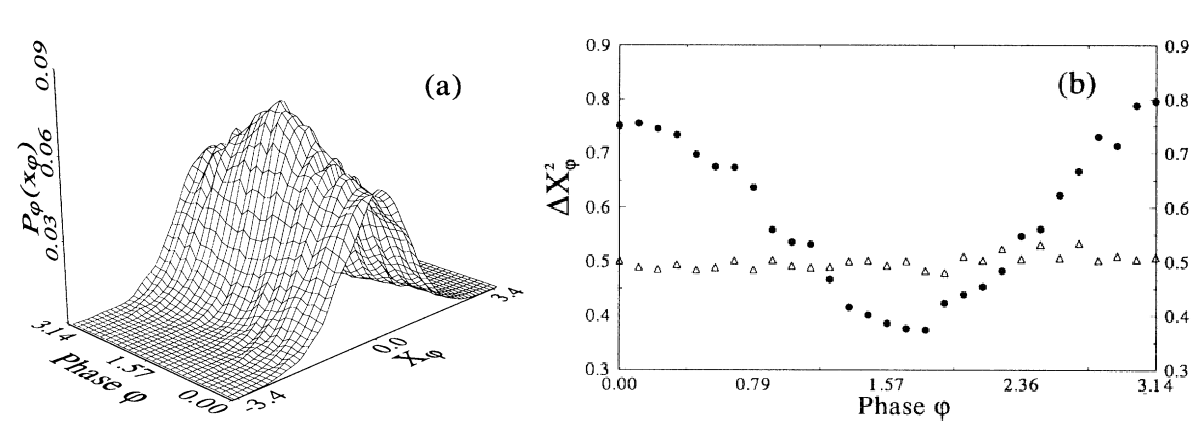
\includegraphics[width=350px,height=138px]{Figures/SmitheyProbabilityDistributionResults.png}%
\caption{Experimental data obtained by Smithey et. al. Show in a) is the marginal distribution of $x_\phi$, of $P_\phi{x_\phi,p_\phi}$, as a function of the local oscillators' swept phase. Panel b) shows the fluctuations of the position quadrature as a function of the local oscillator phase. The near-constant value of .5 for the triangular markers is indicative of vacuum fluctuations (whose variance is constant over the parameter space formed by $x_\phi$ and $p_\phi$). Similarly, the sinusoidal variation of the fluctuations in $x_\phi$, exemplified by the circular markers, is indicative of quadrature squeezing of the vacuum field. Portions of the data which fall significantly below .5 are indicative of the squeezing of the position quadrature. Portions of the data which lie significantly above .5 indicate squeezing of the momentum quadrature.}%
\label{SPDR}%
\end{figure}